\documentclass[10pt]{article}
\usepackage[polish]{babel}
\usepackage[utf8]{inputenc}
\usepackage[T1]{fontenc}
\usepackage{amsmath}
\usepackage{amsfonts}
\usepackage{amssymb}
\usepackage[version=4]{mhchem}
\usepackage{stmaryrd}
\usepackage{graphicx}
\usepackage[export]{adjustbox}
\graphicspath{ {./images/} }
\usepackage{bbold}

\title{LIGA MATEMATYCZNA \\
 im. Zdzisława Matuskiego GRUDZIEŃ 2013 \\
 SZKOŁA PONADGIMNAZJALNA }

\author{}
\date{}


\begin{document}
\maketitle
\section*{ZADANIE 1.}
Na płaszczyźnie danych jest siedem prostych. Wykaż, że kąt pomiędzy pewnymi dwiema prostymi, spośród danych, jest mniejszy niż \(26^{\circ}\).

\section*{ZADANIE 2.}
W koła wpisano liczby w taki sposób, że suma liczb w każdych trzech stycznych kołach jest równa 2013. Oblicz sumę liczb w kołach położonych w wierzchołkach trójkąta.\\
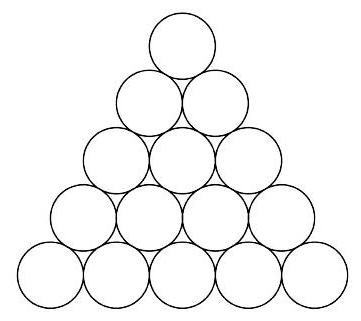
\includegraphics[max width=\textwidth, center]{2024_11_21_24f84c87756b38f2c616g-1}

\section*{ZADANIE 3.}
Znajdź liczbę sześciocyfrową \(\overline{a b c d e f}\) wiedząc, że liczby trzycyfrowe \(\overline{a b c}, \overline{c d e}\) są sześcianami, a liczby \(\overline{b c d} \mathrm{i} \overline{d e f}\) są kwadratami pewnych liczb naturalnych.

\section*{ZADANIE 4.}
Wyznacz wszystkie funkcje \(f: \mathbb{R} \rightarrow \mathbb{R}\) spełniające równość

\[
f(x-|x|)+f(x+|x|)=x
\]

dla każdej liczby rzeczywistej \(x\).

\section*{ZADANIE 5.}
Rozwiąż równanie

\[
\frac{1}{a}+\frac{2}{a b}+\frac{3}{a b c}=1
\]

w zbiorze liczb całkowitych dodatnich.


\end{document}